%% [Stats Project]

%% ================ load packages =============================================================
\documentclass[10pt, twoside]{article}
\usepackage[utf8]{inputenc}
\usepackage{titling, titlesec}
\usepackage{fancyhdr}
\usepackage{amsmath, amsthm, amssymb, array, calc}
\usepackage{thmtools}
\usepackage[a4paper,width=16cm,height=20cm,headheight=23pt,left=2.25cm,right=2.25cm]{geometry}
% a4paper,margin=15mm,headsep=5pt
% width=16cm,height=20.5cm,left=2.5cm,right=2.5cm
\usepackage{tabu, colortbl}
\usepackage[table]{xcolor}
\usepackage{graphicx}
\usepackage[cache=false]{minted}
\usepackage{xpatch}
\usepackage{blindtext}
\usepackage{fancyhdr}
\usepackage{bold-extra}
\usepackage{fontawesome}
\usepackage[hidelinks]{hyperref}

\let\orighref\href
\renewcommand{\href}[2]{\orighref{#1}{#2\,\faExternalLink}}

\raggedbottom
\graphicspath{{./figures/}}
\setlength\textwidth{6.5in}
\setlength\textheight{8.68in}

\xpatchcmd{\minted}{\VerbatimEnvironment}{\VerbatimEnvironment\let\itshape\relax}{}{}
\xpatchcmd{\minted}{\VerbatimEnvironment}{\VerbatimEnvironment\let\bfseries\relax}{}{}
\usemintedstyle{bw}

\pagestyle{fancy}
\renewcommand{\subsectionmark}[1]{\markboth{#1}{}}
\fancyhf{}
\fancyhead[LE,RO]{\raisebox{-0.5cm}{\filcenter\scshape\leftmark}}
\fancyhead[RE,LO]{\raisebox{-0.5cm}{\footnotesize\thepage}}
\renewcommand{\headrulewidth}{0pt}
\fancypagestyle{plain}{\fancyhead{}\renewcommand{\headrulewidth}{0pt}}
\titleformat{\section}[hang]{\filcenter\scshape\normalsize}{}{1pt}{}
\titleformat{\subsection}[hang]{\filcenter\scshape\LARGE}{}{1pt}{}

%% ================ TITLE =====================================================================
%\setlength{\droptitle}{6cm}
\title{Predicting Human Activity}
\author{Michael Šòdéké}
\date{\vspace{-14ex}}

\begin{document}
\maketitle

%% ================ ABSRACT ===================================================================
%% [0-main] block ...
%% -------------------------------------------------------------------------------------------\
\noindent\rule[-2.0\baselineskip]{\linewidth}{0.1pt}
\vspace{-3ex}
\begin{center}
\subsection{abstract}
\vspace{-3ex}
\end{center}
%% -------------------------------------------------------------------------------------------|

%% [B-paragraph] block ...
%% -------------------------------------------------------------------------------------------\
\noindent
\textbf{Background} \\
Traditionally, \textbf{Human Activity Recognition} has focused on predicting \emph{which} activity was
performed at a specific point in time. However, researchers at Groupware focused on
investigating \emph{how well} an activity was performed by the wearer. Six young participants
between 20-28 years were asked to perform a series of five activities to assist Groupware
with this investigation.
\smallskip

\noindent
\textbf{Model Selection} \\
The goal of \textsc{case i} was to select a model function appropriate for predicting the manner in
which participants perfored a series of dumbbell exercises. It turned out that the Random Forest
algorithm (with all covariates) performed the best out of the four, with an out of sample error
(OSE) of $0.0012$.
\smallskip

\noindent
\textbf{Random Forest Prediction} \\
\textsc{case ii} focused on employing the Random Forest algorthm selected in \textsc{case i} for predicting
the manner in which participants perfomred a certain activity. A score of $20/20$ was receieved after
applying prediction results on the quiz.
\smallskip

\vspace{-5.5ex}
\noindent\rule[-2.0\baselineskip]{\linewidth}{0.1pt}
%% -------------------------------------------------------------------------------------------|

\vspace{6ex}

%% ================ BACKGROUND ================================================================
%% [0-main] block ...
%% -------------------------------------------------------------------------------------------\
\begin{center}
\subsection{background}
\vspace{-3ex}
\end{center}
%% -------------------------------------------------------------------------------------------|

%% [B-paragraph] block ...
%% -------------------------------------------------------------------------------------------\
\noindent
\textbf{Human Activity Recognition} has gained attention from the computing research community.
\textsc{har} has many potential applications, such as: elderly monitoring, life log systems for
monitoring energy expenditure and for supporting weight-loss programs, and digital assistants
for weight lifting exercises.
\smallskip

Traditionally, \textsc{har} has focused on predicting \emph{which} activity was performed at a specific
point in time. However, researchers at Groupware focused on investigating \textsc{how well} an
activity was performed by the wearer. Six young participants between 20-28 years performed
"one set of 10 repetitions of the Unilateral Dumbbell Biceps Curl in five different fashions".
These performances are classified as: exactly according to the specification (Class A),
throwing the elbows to the front (Class B), lifting the dumbbell only halfway (Class C),
lowering the dumbbell only halfway (Class D) and throwing the hips to the front (Class E).
\href{http://web.archive.org/web/20161224072740/http:/groupware.les.inf.puc-rio.br/har}{Read more here  }
\bigskip
%% -------------------------------------------------------------------------------------------|

%% ================ CASE 1 ====================================================================
%% [0-main] block ...
%% -------------------------------------------------------------------------------------------\
\begin{center}
\section{CASE I: MODEL SELECTION}
\vspace{-3ex}
\end{center}
%% -------------------------------------------------------------------------------------------|

%% [B-paragraph] block ...
%% -------------------------------------------------------------------------------------------\
\noindent
\blindtext
\bigskip
%% -------------------------------------------------------------------------------------------|

%% [A-title] block ...
%% -------------------------------------------------------------------------------------------\
\begin{center}
\subsection{hypothesis}
\vspace{-3ex}
\end{center}
%% -------------------------------------------------------------------------------------------|

%% [B-paragraph] block ...
%% -------------------------------------------------------------------------------------------\
\noindent
One thing that people regularly do is quantify how much of a particular activity they
do, but they rarely quantify how well they do it. Six young participants between 20-28 years
performed "one set of 10 repetitions of the Unilateral Dumbbell Biceps Curl in five
different fashions". The goal of this report is to predict the manner in which each exercise
was performed. \emph{So, can machine learning be used to predict correct and incorrect movements
for an exercise to help new gym-goers improve their workouts}? In other words, \emph{can machine
learning technology be used to create an A.I. fitness coach}? 
\bigskip
%% -------------------------------------------------------------------------------------------|

%% [A-title] block ...
%% -------------------------------------------------------------------------------------------\
\begin{center}
\subsection{data engineering}
\vspace{-3ex}
\end{center}
%% -------------------------------------------------------------------------------------------|

%% [B-paragraph] block ...
%% -------------------------------------------------------------------------------------------\
\noindent
\href{http://web.archive.org/web/20161224072740/http:/groupware.les.inf.puc-rio.br/har}{A training and testing set were downloaded from Groupware  }.
Upon inspection of the covariates, some have missing values. The R-script file
\textbf{1-C1 dataEng.r} takes care of this issue by eliminating covariates with missing values
and any redundant covariates that are not appropriate for constructing the model. In
addition, the training set is partitioned into a 60\% training and 40\% testing set. Cross
validation will be used only on the sub training set.
\bigskip
%% -------------------------------------------------------------------------------------------|

%% [C-code] block ...
%% -------------------------------------------------------------------------------------------\
\definecolor{lightgrey}{rgb}{0.972,0.972,0.972}
\begin{minted}[linenos=false, bgcolor=lightgrey, fontfamily=qcr, fontsize=\footnotesize]{r}
message("\n\n | [1.] downloading data via URL link...")
message(" --------------------------------------------------------------------")
trnUrl <- "https://d396qusza40orc.cloudfront.net/predmachlearn/pml-training.csv"
tstUrl <- "https://d396qusza40orc.cloudfront.net/predmachlearn/pml-testing.csv"
download.file(trnUrl, destfile="CrossFitData/fitTrain.csv", method = "curl", mode="wb")
download.file(tstUrl, destfile="CrossFitData/fitTest.csv", method = "curl", mode="wb")
print(list.files("./CrossFitData"))
pause()
\end{minted}
%% -------------------------------------------------------------------------------------------|

%% [C-code] block ...
%% -------------------------------------------------------------------------------------------\
\definecolor{lightgrey}{rgb}{0.972,0.972,0.972}
\begin{minted}[linenos=false, bgcolor=lightgrey, fontfamily=qcr, fontsize=\footnotesize]{r}
message("\n\n | [1.2] reading datasets...")
message(" --------------------------------------------------------------------")
file1 <- "./CrossFitData/fitTrain.csv"
file2 <- "./CrossFitData/fitTest.csv"
df.trn <- read.csv(file1)
df.tst <- read.csv(file2)
pause()
\end{minted}
%% -------------------------------------------------------------------------------------------|

%% [C-code] block ...
%% -------------------------------------------------------------------------------------------\
\definecolor{lightgrey}{rgb}{0.972,0.972,0.972}
\begin{minted}[linenos=false, bgcolor=lightgrey, fontfamily=qcr, fontsize=\footnotesize]{r}
message("\n\n | [1.3] cleaning datasets...")
message(" --------------------------------------------------------------------")
# check data summary
message("\t\n\n\n || [1.3.1] checking data summary...")
df.trn %>% str()
df.tst %>% str()
pause()
# convert features to lower case
message("\t\n\n\n || [1.3.2] converting features to lower case...")
colnames(df.trn) <- str_to_lower(colnames(df.trn))
colnames(df.tst) <- str_to_lower(colnames(df.tst))
pause()
\end{minted}
%% -------------------------------------------------------------------------------------------|

%% [C-code] block ...
%% -------------------------------------------------------------------------------------------\
\definecolor{lightgrey}{rgb}{0.972,0.972,0.972}
\begin{minted}[linenos=false, bgcolor=lightgrey, fontfamily=qcr, fontsize=\footnotesize]{r}
# check for na values in training set
message("\t\n\n\n || [1.3.3] checking for na values in training set...")
columns.trn1 <- matrix(colnames(df.trn))
datatype.trn1 <- matrix( sapply( columns.trn1,function(x){ class( df.trn[,x] ) } ) )
check.nas1 <- matrix( sapply( columns.trn1,function(x){ sum(is.na( df.trn[,x] )*1) } ) )
info1 <- cbind(columns.trn1,datatype.trn1,check.nas1)
colnames(info1) <- c("name","type","na")
info1 %>% head(30) %>% print()
pause()
# check for na values in testing set
message("\t\n\n\n || [1.3.4] checking for na values in testing set...")
columns.tst1 <- matrix(colnames(df.tst))
datatype.tst1 <- matrix( sapply( columns.tst1,function(x){ class( df.tst[,x] ) } ) )
check.nas2 <- matrix( sapply( columns.tst1,function(x){ sum(is.na( df.tst[,x] )*1) } ) )
info2 <- cbind(columns.tst1,datatype.tst1,check.nas2)
colnames(info2) <- c("name","type","na")
info2 %>% head(30) %>% print()
pause()
\end{minted}
%% -------------------------------------------------------------------------------------------|

%% [C-code] block ...
%% -------------------------------------------------------------------------------------------\
\definecolor{lightgrey}{rgb}{0.972,0.972,0.972}
\begin{minted}[linenos=false, bgcolor=lightgrey, fontfamily=qcr, fontsize=\footnotesize]{r}
# remove na values
message("\t\n\n\n || [1.3.5] removing na values...")
srch1 <- data.frame(info1)$na == 0
srch2 <- data.frame(info2)$na == 0
pause()
# recheck for na values in training set
message("\t\n\n\n || [1.3.6] rechecking for na values in training set...")
columns.trn2 <- columns.trn1[srch1]
datatype.trn2 <- matrix( sapply( columns.trn2,function(x){ class( df.trn[,x] ) } ) )
check.nas3 <- matrix( sapply( columns.trn2,function(x){ sum(is.na( df.trn[,x] )*1) } ) )
info3 <- cbind(columns.trn2,datatype.trn2,check.nas3)
colnames(info3) <- c("name","type","na")
info3 %>% head(30) %>% print()
pause()
\end{minted}
%% -------------------------------------------------------------------------------------------|

%% [C-code] block ...
%% -------------------------------------------------------------------------------------------\
\definecolor{lightgrey}{rgb}{0.972,0.972,0.972}
\begin{minted}[linenos=false, bgcolor=lightgrey, fontfamily=qcr, fontsize=\footnotesize]{r}
# recheck for na values in testing set
message("\t\n\n\n || [1.3.7] rechecking for na values in testing set...")
columns.tst2 <- columns.tst1[srch2]
datatype.tst2 <- matrix( sapply( columns.tst2,function(x){ class( df.tst[,x] ) } ) )
check.nas4 <- matrix( sapply( columns.tst2,function(x){ sum(is.na( df.tst[,x] )*1) } ) )
info4 <- cbind(columns.tst2,datatype.tst2,check.nas4)
colnames(info4) <- c("name","type","na")
info4 %>% head(30) %>% print()
pause()
# check character type predictors in training set
message("\t\n\n\n || [1.3.8] checking character type predictors in training set...")
df.trn2 <- df.trn[,columns.trn2]
srch3 <- matrix( sapply( colnames(df.trn2),function(x){ is.character( df.trn2[,x] ) } ) )
df.ch <- df.trn2[,srch3]
str(df.ch)
srch4 <- matrix( sapply( colnames(df.ch),
        function(x){ if (sum((df.trn2[,x] == "")*1) > 1 ){ TRUE }else{ FALSE } } ) )
newTypes <- matrix( sapply( colnames(df.ch[,srch4]),
        function(x){ as.numeric( df.trn2[,x] ) } ), ncol=ncol(df.ch[,srch4]) )
df.ch[,srch4] <- newTypes
df.trn2[,colnames(df.ch[,srch4])] <- newTypes
df.trn2 %>% str()
pause()
\end{minted}
%% -------------------------------------------------------------------------------------------|

%% [C-code] block ...
%% -------------------------------------------------------------------------------------------\
\definecolor{lightgrey}{rgb}{0.972,0.972,0.972}
\begin{minted}[linenos=false, bgcolor=lightgrey, fontfamily=qcr, fontsize=\footnotesize]{r}
# check character type predictors in testing set
message("\t\n\n\n || [1.3.9] checking character type predictors in testing set...")
df.tst2 <- df.tst[,columns.tst2]
srch5 <- matrix( sapply( colnames(df.tst2),function(x){ is.character( df.tst2[,x] ) } ) )
df.ch <- df.trn2[,srch5]
df.ch %>% str()
srch6 <- matrix( sapply( colnames(df.ch),
        function(x){ if (sum((df.tst2[,x] == "")*1) > 1 ){ TRUE }else{ FALSE } } ) )
newTypes <- matrix( sapply( colnames(df.ch[,srch6]),
        function(x){ as.numeric( df.tst2[,x] ) } ), ncol=ncol(df.ch[,srch6]) )
df.ch[,srch6] <- newTypes
df.tst2[,colnames(df.ch[,srch6])] <- newTypes
df.tst2 %>% str()
pause()
# recheck for na values in training set
message("\t\n\n\n || [1.3.10] rechecking for na values in training set...")
columns.trn3 <- matrix(colnames(df.trn2))
datatype.trn3 <- matrix( sapply( columns.trn3,function(x){ class( df.trn2[,x] ) } ) )
check.nas3 <- matrix( sapply( columns.trn3,function(x){ sum(is.na( df.trn2[,x] )*1) } ) )
info5 <- cbind(columns.trn3,datatype.trn3,check.nas3)
colnames(info5) <- c("name","type","na")
info5 %>% head(30) %>% print()
pause()
\end{minted}
%% -------------------------------------------------------------------------------------------|

%% [C-code] block ...
%% -------------------------------------------------------------------------------------------\
\definecolor{lightgrey}{rgb}{0.972,0.972,0.972}
\begin{minted}[linenos=false, bgcolor=lightgrey, fontfamily=qcr, fontsize=\footnotesize]{r}
info5 %>% head(30) %>% print()
pause()
# remove na values
message("\t\n\n\n || [1.3.11] remove na values...")
srch7 <- data.frame(info5)$na == 0
pause()
# recheck for na values in training set
message("\t\n\n\n || [1.3.12] rechecking for na values in training set...")
columns.trn4 <- columns.trn3[srch7]
datatype.trn4 <- matrix( sapply( columns.trn4,function(x){ class( df.trn2[,x] ) } ) )
check.nas4 <- matrix( sapply( columns.trn4,function(x){ sum(is.na( df.trn2[,x] )*1) } ) )
info6 <- cbind(columns.trn4,datatype.trn4,check.nas4)
colnames(info6) <- c("name","type","na")
info6 %>% head(30) %>% print()
pause()
\end{minted}
%% -------------------------------------------------------------------------------------------|

%% [C-code] block ...
%% -------------------------------------------------------------------------------------------\
\definecolor{lightgrey}{rgb}{0.972,0.972,0.972}
\begin{minted}[linenos=false, bgcolor=lightgrey, fontfamily=qcr, fontsize=\footnotesize]{r}
# check columns in training and testing set
message("\t\n\n\n || [1.3.13] checking columns in training and testing set...")
df.trn3 <- df.trn2[,columns.trn4]
df.trn3 %>% str()
df.tst2 %>% str()
colnames(df.trn3) == colnames(df.tst2)
pause()
# fix date formating
message("\t\n\n\n || [1.3.14] fixing date formating...")
df.trn3$cvtd_timestamp <- dmy_hm(df.trn3$cvtd_timestamp)
df.tst2$cvtd_timestamp <- dmy_hm(df.tst2$cvtd_timestamp)
pause()
\end{minted}
%% -------------------------------------------------------------------------------------------|

%% [C-code] block ...
%% -------------------------------------------------------------------------------------------\
\definecolor{lightgrey}{rgb}{0.972,0.972,0.972}
\begin{minted}[linenos=false, bgcolor=lightgrey, fontfamily=qcr, fontsize=\footnotesize]{r}
# prepare training set
message("\t\n\n\n || [1.3.15] preparing training set...")
df.trn3$classe <- factor(df.trn3$classe)
df.trn3 <- df.trn3[,-c(1:7)]
df.trn4 <- data.frame(df.trn3)
srch <- createDataPartition(df.trn4$classe, p = 3/4)[[1]]
trn <- df.trn4[srch,]
trn %>% str()
View(trn)
pause()
# prepare pre testing set
message("\t\n\n\n || [1.3.16] preparing [pre] testing set...")
tst.pre <- df.trn4[-srch,]
tst.pre %>% str()
View(tst.pre)
pause()
\end{minted}
%% -------------------------------------------------------------------------------------------|

%% [C-code] block ...
%% -------------------------------------------------------------------------------------------\
\definecolor{lightgrey}{rgb}{0.972,0.972,0.972}
\begin{minted}[linenos=false, bgcolor=lightgrey, fontfamily=qcr, fontsize=\footnotesize]{r}
# prepare final testing set
message("\t\n\n\n || [1.3.17] preparing [final] testing set...")
df.tst2 <- df.tst2[,-c(1:7)]
#df.tst2$problem_id <- NULL
tst.final <- data.frame(df.tst2)
tst.final %>% str()
View(tst.final)
pause()
\end{minted}
%% -------------------------------------------------------------------------------------------|

%% [A-title] block ...
%% -------------------------------------------------------------------------------------------\
\begin{center}
\subsection{descriptive statistics}
\vspace{-3ex}
\end{center}
%% -------------------------------------------------------------------------------------------|

%% [B-paragraph] block ...
%% -------------------------------------------------------------------------------------------\
\noindent
The goal of Groupware is to investigate how well each participant performed each dumbbell
exercise. In \textsc{figure 1.}, descriptive statistics show both Adelmo and Jeremy have the best
performance out of the six participants. The R-script file \textbf{2-C1 descriptiveStats.r} performs
additional data transformations to construct the desired plots.
\bigskip
%% -------------------------------------------------------------------------------------------|

%% [D2-result-image] block ...
%% -------------------------------------------------------------------------------------------\
\begin{figure}[H]
\centering
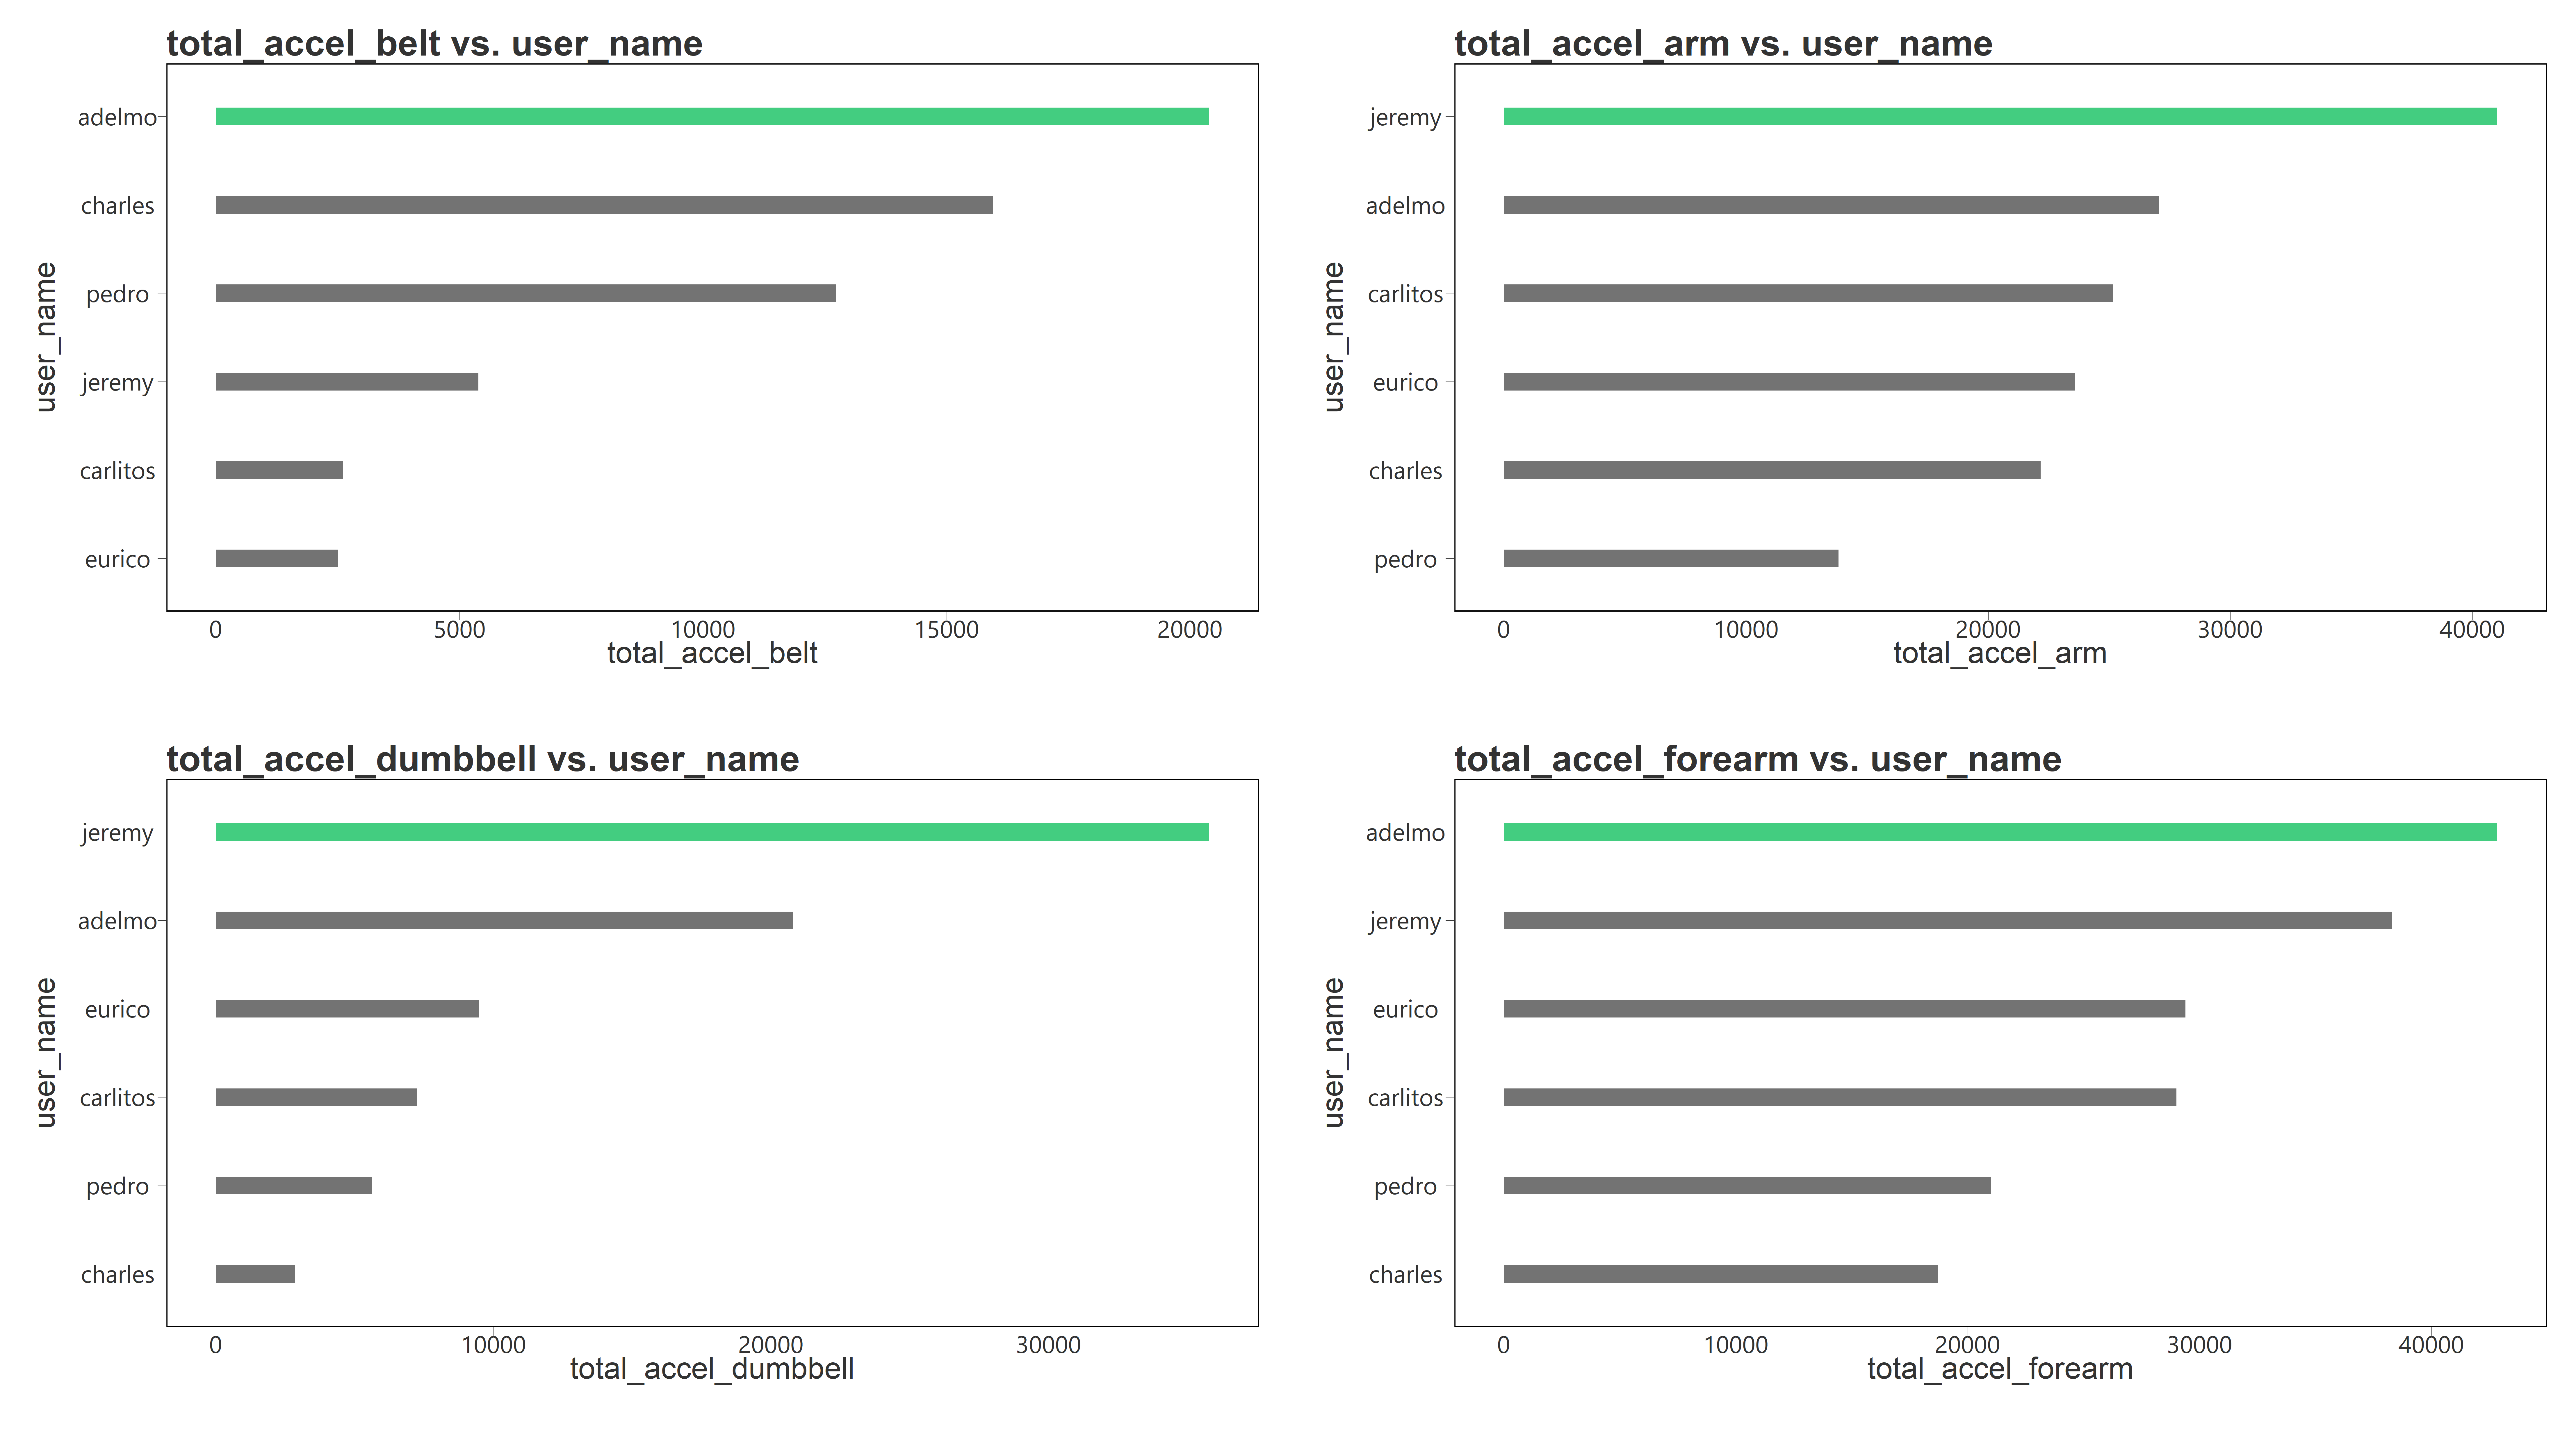
\includegraphics[scale=0.359]{plot1}
\caption{}
\end{figure}
%% -------------------------------------------------------------------------------------------|

%% [A-title] block ...
%% -------------------------------------------------------------------------------------------\
\begin{center}
\subsection{prediction study design: defining error rate}
\vspace{-3ex}
\end{center}
%% -------------------------------------------------------------------------------------------|

%% [B-paragraph] block ...
%% -------------------------------------------------------------------------------------------\
\noindent
The first step in Prediction Study Design is to define the error rate. For now
Accuracy will be employed to determine which model function is best appropriate for
answering the above hypothesis. The R-script file \textbf{3-C1 predStudyDesign.r} will assist
in definging the error rate and in K-fold cross validation.
\smallskip

\begin{equation*}
\begin{aligned}
ER_{accuracy} = \frac{TP + TN}{TP + TN + FP + FN}
\end{aligned}
\end{equation*}
\bigskip
%% -------------------------------------------------------------------------------------------|

%% [A-title] block ...
%% -------------------------------------------------------------------------------------------\
\begin{center}
\subsection{prediction study design: k-fold cross validation}
\vspace{-3ex}
\end{center}
%% -------------------------------------------------------------------------------------------|

%% [B-paragraph] block ...
%% -------------------------------------------------------------------------------------------\
\noindent
Cross validation is used on the sub training set, which will be partioned repeatedly based
on $K = 5$ folds into another 60\% training and 40\% test set. 
\smallskip

Four models are trained with K-fold cross validation and plotted to determine accuracy and
examine error rates. The first model employes a \textbf{CART} algorithm with all covariates, while
the second employes a \textbf{Random Forest} algorithm with all covariates. The third and fourth models
are the same as the previous two models, but with selected covariates: \textbf{classe}, \textbf{total accel belt},
\textbf{total accel arm}, \textbf{total accel dumbbell}, and \textbf{total accel forearm}.
\bigskip
%% -------------------------------------------------------------------------------------------|

%% [C-code] block ...
%% -------------------------------------------------------------------------------------------\
\definecolor{lightgrey}{rgb}{0.972,0.972,0.972}
\begin{minted}[linenos=false, bgcolor=lightgrey, fontfamily=qcr, fontsize=\footnotesize]{r}
# perform k-fold cross validation--[CART algorithm]
message("\t\n\n\n || [3.0.2] performing [K-FOLD] cross validation--[CART algorithm]...")
set.seed(16033)
no_cores <- detectCores() - 1
cl <- makePSOCKcluster(no_cores)
registerDoParallel(cl)
Bcart_ <- 0

tic()
stash("Bcart_", {
  Sys.sleep(5)
  Bcart_ <- train(classe ~ .,method="rpart",data=trn,
      trControl=trainControl(method="cv",number=5,p=0.60,allowParallel=T))
})
toc()

Bcart_ %>% print()
pause()
\end{minted}
%% -------------------------------------------------------------------------------------------|

%% [C-code] block ...
%% -------------------------------------------------------------------------------------------\
\definecolor{lightgrey}{rgb}{0.972,0.972,0.972}
\begin{minted}[linenos=false, bgcolor=lightgrey, fontfamily=qcr, fontsize=\footnotesize]{r}
# perform k-fold cross validation--[rf algorithm]
message("\t\n\n\n || [3.0.3] performing [K-FOLD] cross validation--[rf algorithm]...")
Brf_ <- 0

tic()
stash("Brf_", {
  Sys.sleep(5)
  Brf_ <- train(classe ~ .,method="rf",data=trn,
          trControl=trainControl(method="cv",number=5,p=0.60,allowParallel=T))
})
toc()

Brf_ %>% print()
pause()
\end{minted}
%% -------------------------------------------------------------------------------------------|

%% [C-code] block ...
%% -------------------------------------------------------------------------------------------\
\definecolor{lightgrey}{rgb}{0.972,0.972,0.972}
\begin{minted}[linenos=false, bgcolor=lightgrey, fontfamily=qcr, fontsize=\footnotesize]{r}
# perform k-fold cross validation--[CART algorithm] on selected regressors
message("\t\n\n\n || [3.0.4] performing [K-FOLD] cross validation--[CART algorithm]...")
df1 <- trn %>% select(classe,total_accel_belt,total_accel_arm,
                total_accel_dumbbell,total_accel_forearm)
Bcart2_ <- 0

tic()
stash("Bcart2_", {
  Sys.sleep(5)
  Bcart2_ <- train(classe ~ .,method="rpart",data=df1,
       trControl=trainControl(method="cv",number=5,p=0.60,allowParallel=T))
})
toc()

Bcart2_ %>% print()
stopCluster(cl)
registerDoSEQ()
pause()
\end{minted}
%% -------------------------------------------------------------------------------------------|

%% [C-code] block ...
%% -------------------------------------------------------------------------------------------\
\definecolor{lightgrey}{rgb}{0.972,0.972,0.972}
\begin{minted}[linenos=false, bgcolor=lightgrey, fontfamily=qcr, fontsize=\footnotesize]{r}
# perform k-fold cross validation--[rf algorithm] on selected regressors
message("\t\n\n\n || [3.0.5] performing [K-FOLD] cross validation--[rf algorithm]...")
df1 <- trn %>% select(classe,total_accel_belt,total_accel_arm,
          total_accel_dumbbell,total_accel_forearm)
Brf2_ <- 0

tic()
stash("Brf2_", {
  Sys.sleep(5)
  Brf2_ <- train(classe ~ .,method="rf",data=df1,
           trControl=trainControl(method="cv",number=5,p=0.60,allowParallel=T))
})
toc()

Brf2_ %>% print()
pause()
\end{minted}
%% -------------------------------------------------------------------------------------------|

%% [B-paragraph] block ...
%% -------------------------------------------------------------------------------------------\
\noindent
It turns out that the Random Forest algorithm (with all covariates) performed the best out
of the four, with an out of sample error (OSE) of $0.0012$. In addition, \textsc{figure 2.}
shows that reducing covariates for classification algorithms has a negative impact on
performance and increases the error rate.
\bigskip
%% -------------------------------------------------------------------------------------------|

%% [C-code] block ...
%% -------------------------------------------------------------------------------------------\
\definecolor{lightgrey}{rgb}{0.972,0.972,0.972}
\begin{minted}[linenos=false, bgcolor=lightgrey, fontfamily=qcr, fontsize=\footnotesize]{r}
# compare accuracies
message("\t\n\n\n || [3.0.6] comparing accuracies...")
check <- list("|[CART--ALL]|"=Bcart_,"|[CART--selected]|"=Bcart2_,
        "|[RF--ALL]|"=Brf_,"|[RF--selected]|"=Brf2_)
check %>% print()
pause()
\end{minted}
%% -------------------------------------------------------------------------------------------|

%% [C-code] block ...
%% -------------------------------------------------------------------------------------------\
\definecolor{lightgrey}{rgb}{0.972,0.972,0.972}
\begin{minted}[linenos=false, bgcolor=lightgrey, fontfamily=qcr, fontsize=\footnotesize]{r}
> Brf_
Random Forest

14718 samples
   52 predictor
    5 classes: 'A', 'B', 'C', 'D', 'E'

No pre-processing
Resampling: Cross-Validated (5 fold)
Summary of sample sizes: 11775, 11775, 11774, 11773, 11775
Resampling results across tuning parameters:

  mtry  Accuracy   Kappa
   2    0.9915752  0.9893413
  27    0.9915753  0.9893422
  52    0.9821311  0.9773913

Accuracy was used to select the optimal model using the largest value.
The final value used for the model was mtry = 27.
\end{minted}
%% -------------------------------------------------------------------------------------------|


%% [D2-result-image] block ...
%% -------------------------------------------------------------------------------------------\
\begin{figure}[H]
\centering
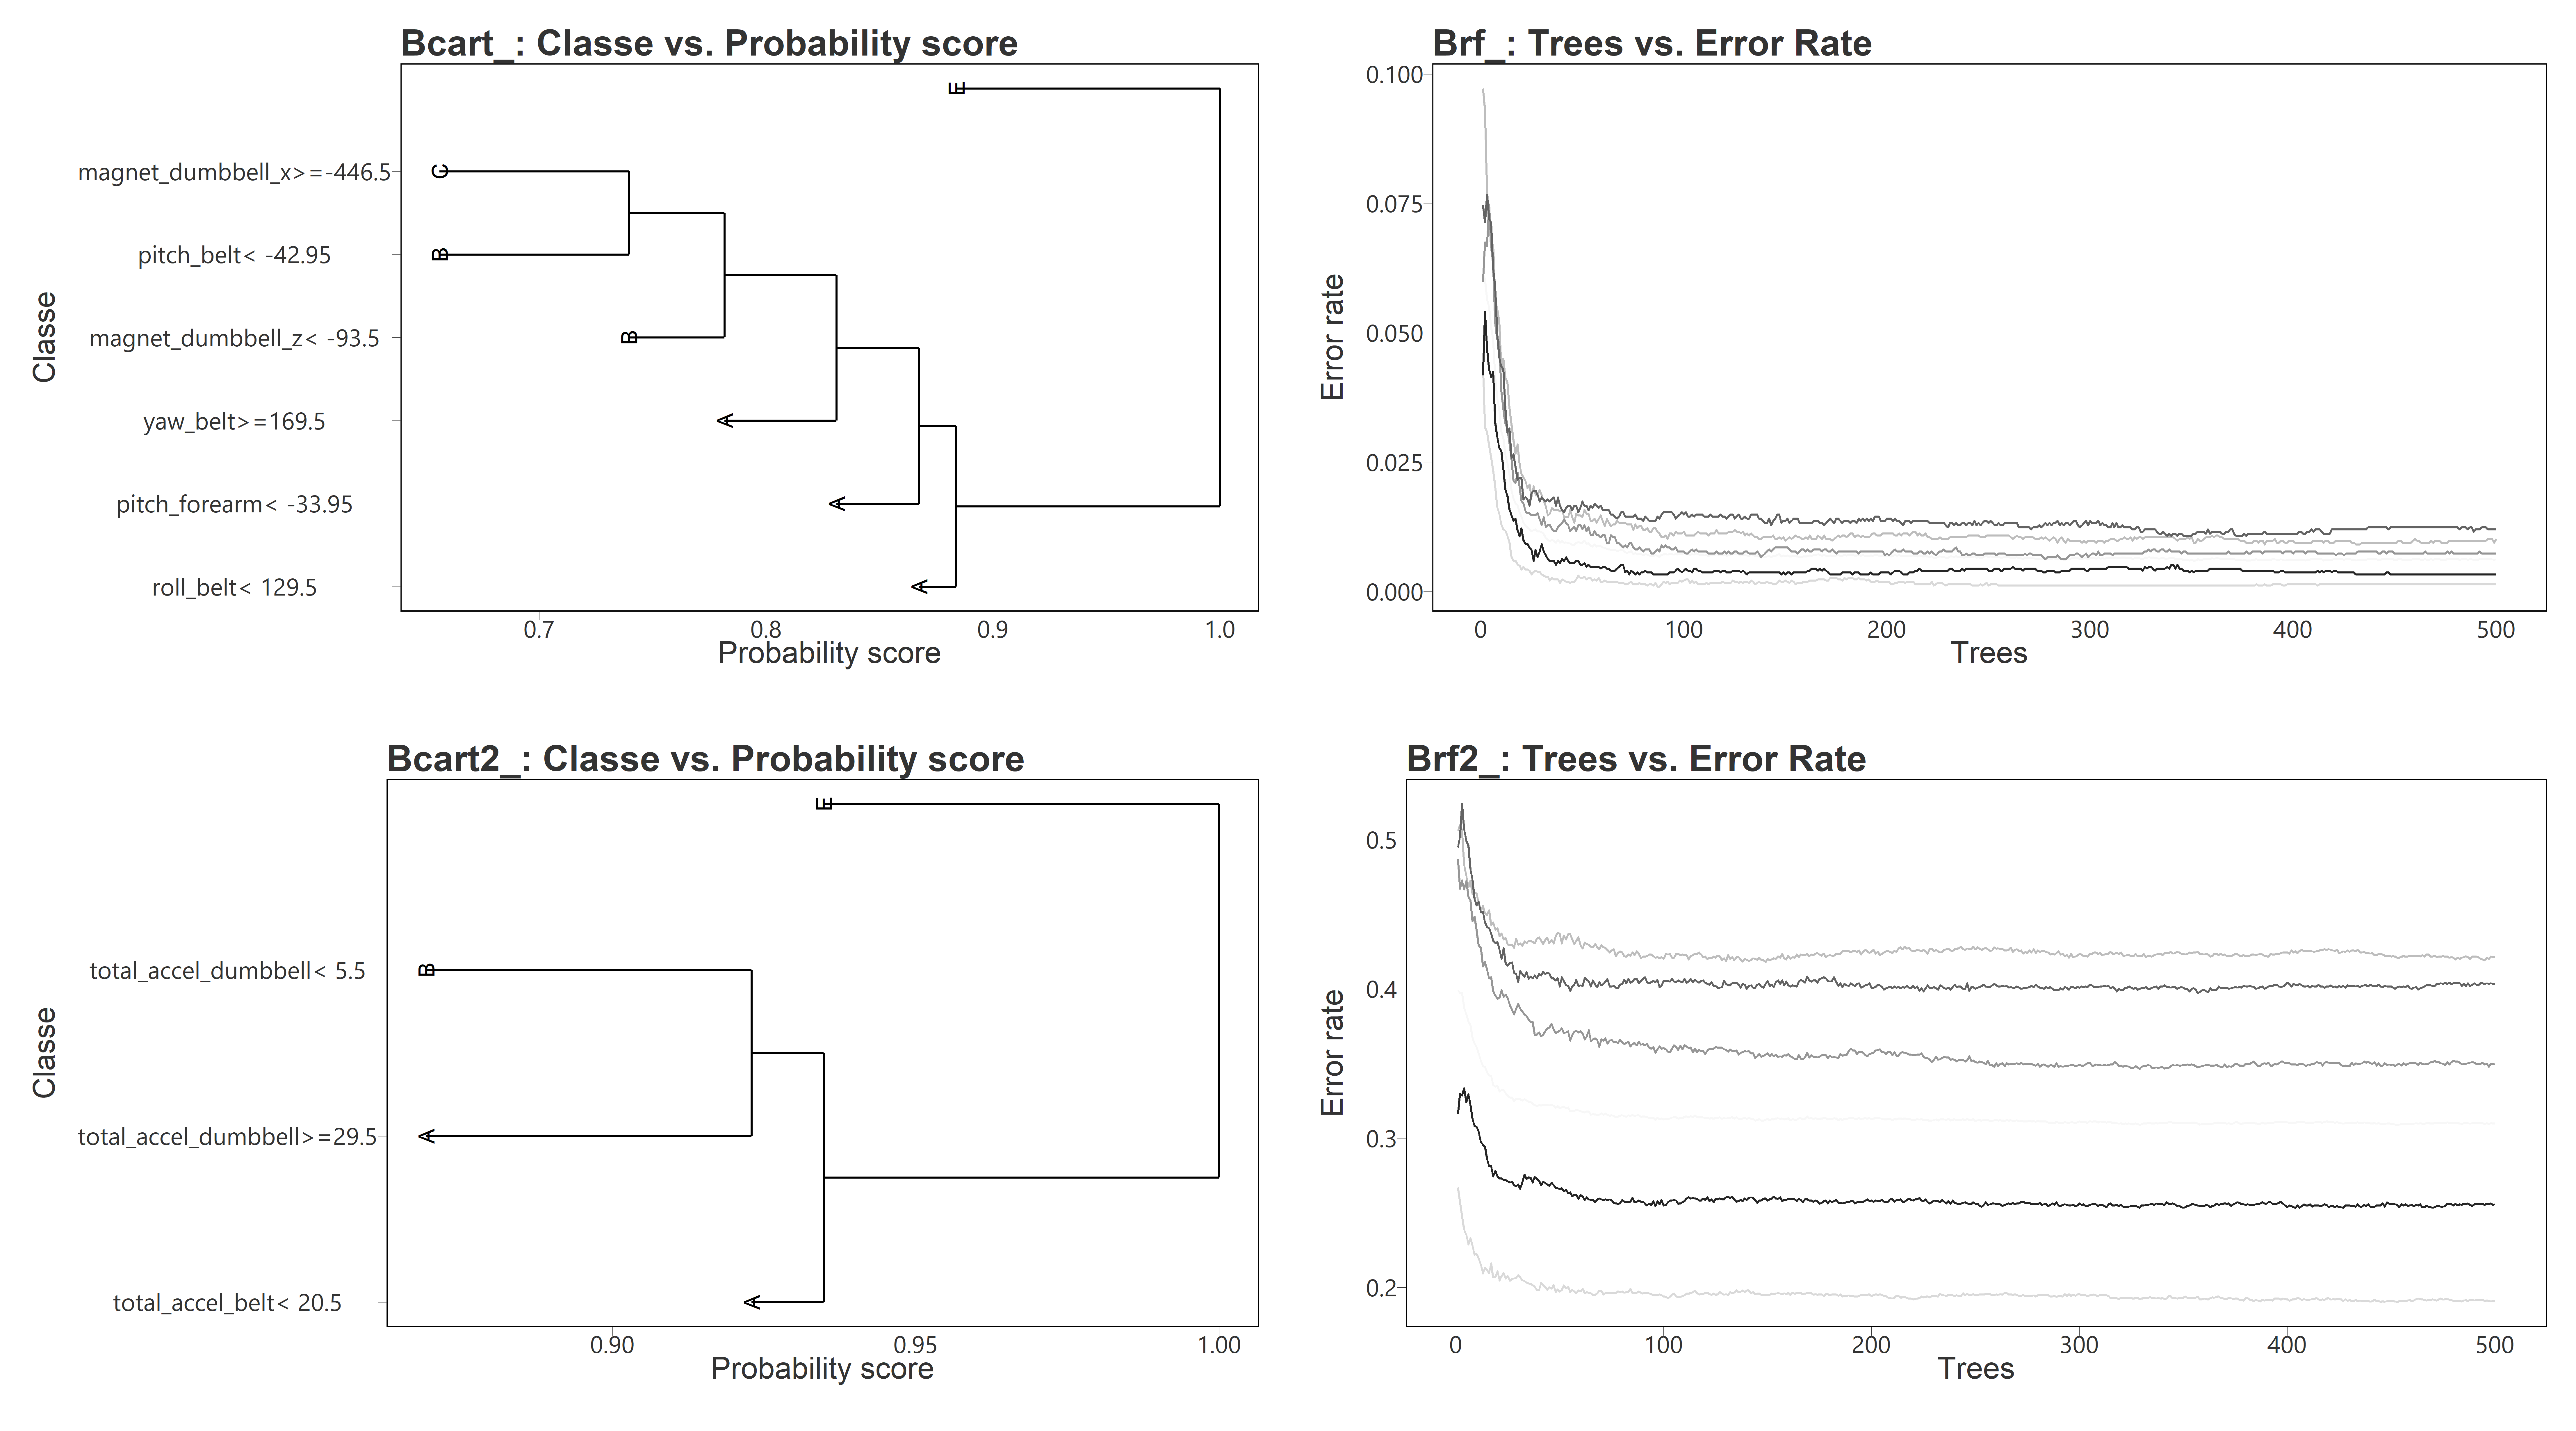
\includegraphics[scale=0.359]{plot2}
\caption{}
\end{figure}
%% -------------------------------------------------------------------------------------------|


\newpage

%% ================ CASE 2 ====================================================================
%% [0-main] block ...
%% -------------------------------------------------------------------------------------------\
\begin{center}
\section{CASE II: RANDOM FOREST PREDICTION}
\vspace{-3ex}
\end{center}
%% -------------------------------------------------------------------------------------------|

%% [B-paragraph] block ...
%% -------------------------------------------------------------------------------------------\
\noindent
\textsc{case ii} focuses on employing the model function selected in \textsc{case i} for predicting the manner
in which participants perfomred a certain activity. The first prediction is based on the
testing set produced when the training set was partitioned. The second prediction is based on
the testing set provided by Groupware. Results from the second prediction is then applied to
the quiz to determine if the predictions were correct. The report ends with a 
discussion on the results and the future of Human Activity Recognition.
\bigskip
%% -------------------------------------------------------------------------------------------|

%% [A-title] block ...
%% -------------------------------------------------------------------------------------------\
\begin{center}
\subsection{prediction}
\vspace{-3ex}
\end{center}
%% -------------------------------------------------------------------------------------------|

%% [B-paragraph] block ...
%% -------------------------------------------------------------------------------------------\
\noindent
The first prediction is conducted on the 40\% testing set, created when the training set
was partitioned. The second prediction is based on the testing set provided by Groupware.
A score of $20/20$ was receieved after applying prediction results on the quiz. The R-script
\textbf{4-C2 prediction.r} performs both predictions and provides the OSE mentioned in \textsc{case i}.
\bigskip
%% -------------------------------------------------------------------------------------------|

%% [C-code] block ...
%% -------------------------------------------------------------------------------------------\
\definecolor{lightgrey}{rgb}{0.972,0.972,0.972}
\begin{minted}[linenos=false, bgcolor=lightgrey, fontfamily=qcr, fontsize=\footnotesize]{r}
message("\n\n | [4.] prediction ...")
message(" --------------------------------------------------------------------")
# predict manner in which participants performed dumbbell exercises
message("\t\n\n\n || [4.0.1] predicting based on [classe] variable in [trn.pre] ...")
y_ <- matrix(predict(Brf_,newdata=tst.pre))
ACC <- confusionMatrix(factor(y_), tst.pre$classe)$overall[1]
OSE <- 1 - ACC
val <- data.frame("accuracy"=ACC,"out.of.sample.error"=OSE); rownames(val) <- NULL
val %>% print()
pause()
# predict manner in which participants performed dumbbell exercises
message("\t\n\n\n || [4.0.1] predicting based on [classe] variable in [trn.final] ...")
y_ <- matrix(predict(Brf_,newdata=tst.final))
y_ %>% print()
pause()
\end{minted}
%% -------------------------------------------------------------------------------------------|

%% [C-code] block ...
%% -------------------------------------------------------------------------------------------\
\definecolor{lightgrey}{rgb}{0.972,0.972,0.972}
\begin{minted}[linenos=false, bgcolor=lightgrey, fontfamily=qcr, fontsize=\footnotesize]{r}
> y_
      [,1]
 [1,] "B"
 [2,] "A"
 [3,] "B"
 [4,] "A"
 [5,] "A"
 [6,] "E"
 [7,] "D"
 [8,] "B"
 [9,] "A"
[10,] "A"
[11,] "B"
[12,] "C"
[13,] "B"
[14,] "A"
[15,] "E"
[16,] "E"
[17,] "A"
[18,] "B"
[19,] "B"
[20,] "B"
\end{minted}
%% -------------------------------------------------------------------------------------------|

%% [A-title] block ...
%% -------------------------------------------------------------------------------------------\
\begin{center}
\subsection{discussion}
\vspace{-3ex}
\end{center}
%% -------------------------------------------------------------------------------------------|

%% [B-paragraph] block ...
%% -------------------------------------------------------------------------------------------\
\noindent
Results from the Random Forest algorithm show promissing results. While A.I. is still at
its infancy, it will develop to a point were \textsc{har} can assist gym-goers with various
exercises. The future of \textsc{har} seems bright. I would suggest more research and development into
\textsc{har} and bioinformatics. With this development, \textsc{har} can inform doctors and device users
of certain body activities and their association with cellular activities. The Random Forest
algorithms seems most applicable for classification predictions of this calibar. However, it
may be replaced by more advanced algorithms of its kind in the future.
%% -------------------------------------------------------------------------------------------|
\end{document}